\chapter{EXPERIMENTAL RESULTS}
The experiments were run on a DELL computer equipped with a 3.6 GHz Intel Xeon processor and a 24 GB RAM.
\section{Example Data Sets}
In these experiments, we used two LC-MS data sets with spiked molecular standards. The first was a metabolomics LC-MS data of mouse liver extract. The second was a proteomics LC-MS data of human urine \cite{christin}.
\begin{itemize}
	\item{ \textbf{Metabolomics data of mouse liver metabolite extract with spiked metabolite standards}}
\end{itemize}


This data was generated in our lab by extracting metabolites from a pooled mouse liver sample using a solvent mixture water:methabol $(v:v = 8:2)$. The metabolite extract was then equally split into 60 aliquots to form 6 sample groups $(G0, G1,\ldots,G5 )$ with (n=10 in each group). Different volumes of a mixture of 48 metabolite standards were spiked in each sample. The concentrations of each metabolite standard spiked in the 6 sample groups were $0 \mu M$, $0.625 \mu M$, $1.25 \mu M$, $2.5 \mu M$, $5 \mu M$  and $10 \mu M$, respectively. All samples were analyzed on a Q Exactive HF Hybrid Quadrupole-Orbitrap Mass Spectrometer equipped with a C18 RP column and a HILIC column configured in parallel. The MS was operated in both positive and negative modes to acquire the full MS and MS/MS spectra for each metabolite. LC-MS data were first analyzed using MetSign software \cite{metsign} for spectrum deconvolution, metabolite assignment and cross-sample peak list alignment.\\

\begin{itemize}
\item{\textbf{Proteomics data of human urine with spiked peptide mixtures} }
\end{itemize}

This publicly available data set was generated from 8 different sample groups with 5 samples in each
group. The data set was introduced in (\cite{christin}). Briefly, a pooled urine sample, collected from 15 healthy females and 35 healthy males over the age range of 26.9 to 72.9 years, was spiked with a tryptic digest (V5111; Promega, Madison, WI) of bovine carbonic anhydrase (C3934, Uniprot entry: P00921; Sigma, Steinheim, Germany), as well as with seven synthetic peptides at eight different dilutions: 6.25, 12.5, 25, 50, 100, 200, 400, and 2000 times dilution. The final data covers peaks with m/z values from 280 to 1500 amu, with a constant resolution of 0.1 amu, and retention times between 30 and 85 min, resulting in a final common peak list of 29,529 features, with 151 of those originating from the added peptides (i.e. biomarkers).

\section{Validation of the proposed MSN algorithm by data classification}


The LC-MS metabolomics data was used to validate the proposed MSN method and its performance was compared with existing normalization methods outlined in Chapter 2. First, we considered groups $G0$ and $G5$ (the easiest case since $G5$ samples were spiked with the highest concentration of each metabolite standard) and normalized the data using the different methods. Next, for each normalized data, we used PLS-DA as a classifier to assign a confidence value showing the likelihood of each metabolite to be a biomarker. Then, using these confidence values and the ground truth, we generated an ROC curve and computed the area under the curve (AUC) within $[0 \ldots 0.1]$. Thus, if all biomarkers (i.e. spiked-in metabolite standards) could be detected with no false positives, then $AUC = 0.1$, else $AUC < 0.1$. Next, to analyze the effect of noise on the different normalization methods, we corrupted one of the samples from $G0$ with multiplicative noise. Specifically, for each metabolite $i$, we modified its peak area using $P'_{i,k}=(1+ \epsilon )P_{i,k}$, where $k$ is the sample to be corrupted, $\epsilon$ is a random number uniformly distributed in the range $[0,U]$ with $U=5\%$, $10 \%$, $15 \% $,and $20 \% $ (the case of noise free samples correspond to U=0). Due to the randomness of the added noise, we repeated this experiment 10 times and reported the mean and standard deviations of the AUC. 

\begin{figure}
	
	\centering
	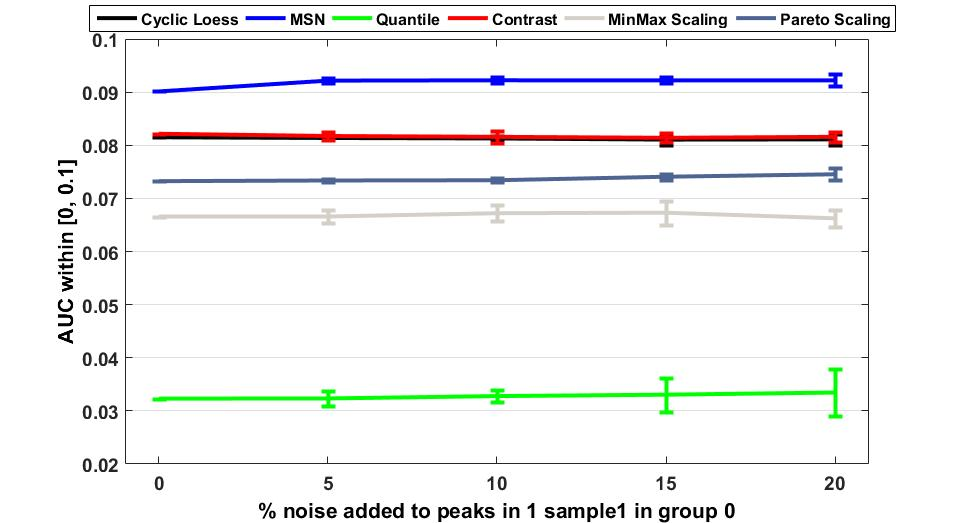
\includegraphics[width=1\textwidth]{ErrorBar_PLSDA_s3}
	\caption{Comparison of the performance of the proposed MSN method to 5 normalization methods when groups G0 and G5 are considered and as we vary the noise level on one sample in G0 in Liver Extraction Data.}
	\label{ErrorBar_PLSDA_s3}
\end{figure}

\begin{figure}
	
	\centering
	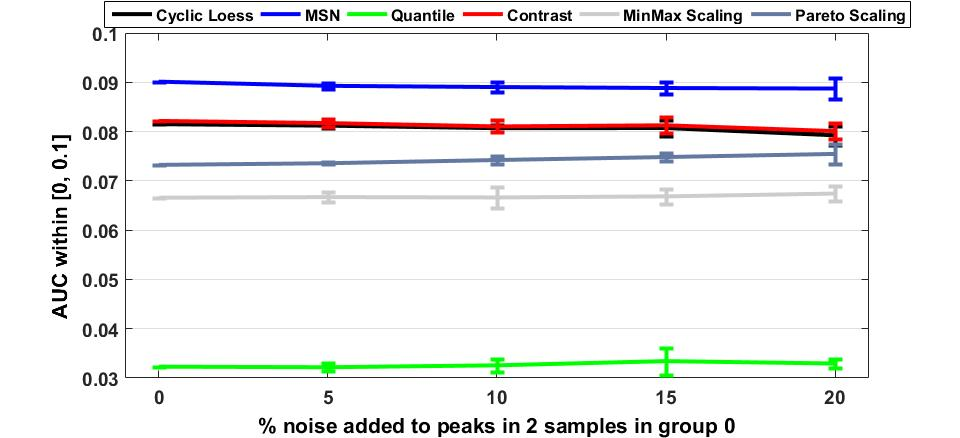
\includegraphics[width=1\textwidth]{ErrorBar_PLSDA_2samples}
	\caption{Comparison of the performance of the proposed MSN method to 5 normalization methods when groups G0 and G5 are considered and as we vary the noise level on two samples in G0 in Liver Extraction Data.}
	\label{ErrorBar_PLSDA_2samples}
\end{figure}

Figure ~\ref{ErrorBar_PLSDA_s3} shows the results obtained by all normalization methods for all 5 levels of added noise. As it can be seen, the proposed MSN normalization is significantly better than all other methods as it has the largest AUC values at all noise levels. Second, the MSN (and most other methods) are robust to noise since the performance does not degrade as noise increases from $0\%$ to $20\%$. Third, we note the small standard deviation indicating the consistency of the results across the multiple runs with different random noise. 

In a second experiment, we added noise to two samples from group $G0$ (i.e. samples 3 and 6) and repeated the same experiment. The results are shown in Figure ~\ref{ErrorBar_PLSDA_2samples} where similar behavior can be concluded. 

We performed multiple other evaluations by adding noise to samples from $G5$ and by considering other groups $G1 \ldots G4$. As expected, the performance degraded as we considered groups containing metabolite standards with less spiked-in concentrations. However, MSN remained as the most robust method and performed significantly better than the other 5 methods. In Figure ~\ref{ErrorBar_PLSDA_2samplesingroup0-3} we show the results when we considered groups G0 and G3 and when two samples from G0 were corrupted by noise. 

\begin{figure}
	
	\centering
	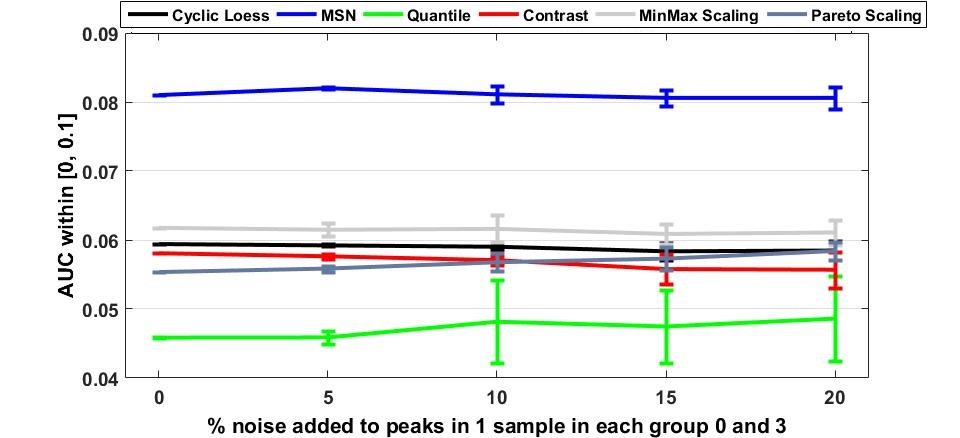
\includegraphics[width=1\textwidth]{ErrorBar_PLSDA_2samplesingroup0-3}
	\caption{Comparison of the performance of the proposed MSN methods to 5 normalization methods when groups G0 and G3 are considered and as we vary the noise level on two samples in G0 in the Liver Extraction Data.}
	\label{ErrorBar_PLSDA_2samplesingroup0-3}
\end{figure}

To analyze the results further, in Figure ~\ref{MZ-data_surfaceOfS3} and ~\ref{RT-data_surfaceOfS3} we display the surface fitted to the potential house-keeping metabolites of sample 3 before and after adding $20\%$ noise. To simplify the visualization of the 3-D surface, Figure ~\ref{MZ-data_surfaceOfS3} displays normalization factor $w_{ij}$ vs. m/z and Figure ~\ref{RT-data_surfaceOfS3} displays $w_{ij}$  vs.  $t_R$. As it can be seen, $w_{ij}$  tends to increase as we add noise. Normalizing by higher values will reduce the effect of noise. 



\begin{figure}
	
	\centering
	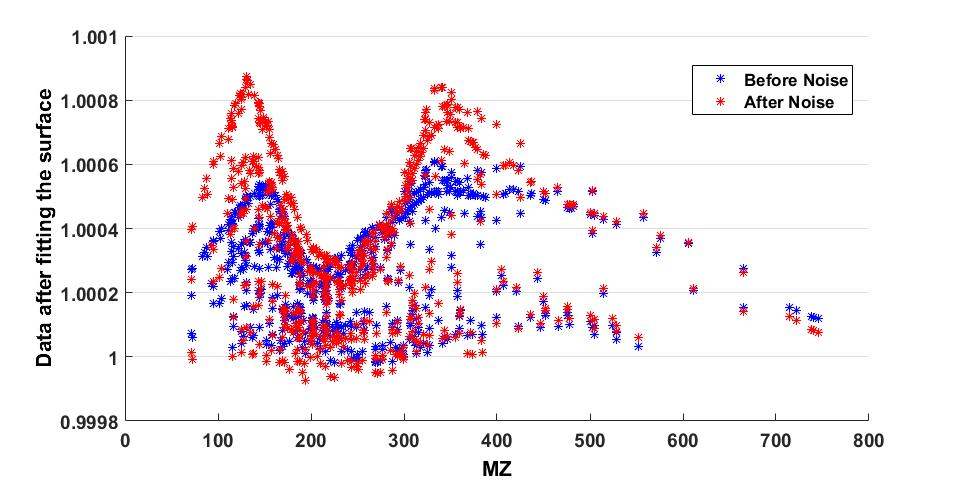
\includegraphics[width=1\textwidth]{MZ-data_surfaceOfS3}
	\caption{Learned normalization factors, as a function of the m/z values, for the potential house-keeping metabolites of sample 3 in $G0$ before and after adding $20\%$ noise in Liver Extraction Data.}
	\label{MZ-data_surfaceOfS3}
\end{figure}

\begin{figure}
	
	\centering
	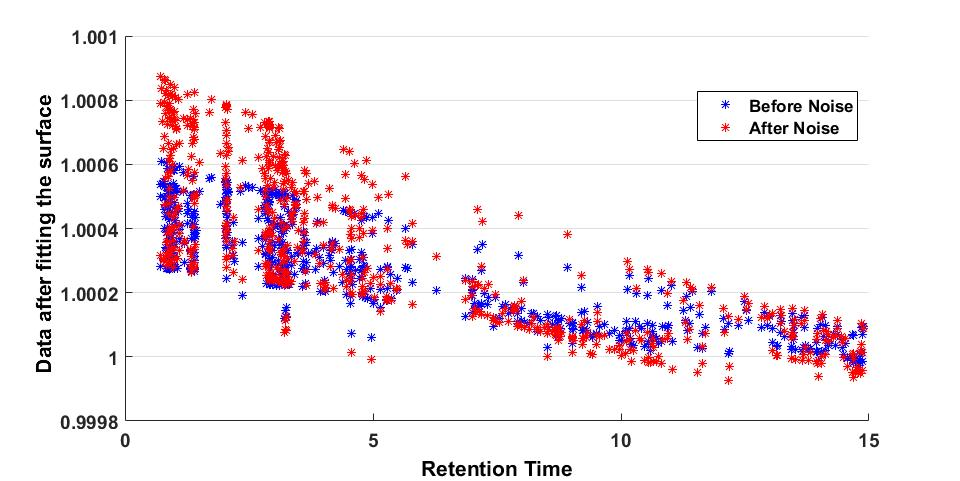
\includegraphics[width=1\textwidth]{RT-data_surfaceOfS3}
	\caption{Learned normalization factors, as a function of the retention time, for the potential house-keeping metabolites of sample 3 in $G0$ before and after adding $20\%$ noise in Liver Extraction Data.}
	\label{RT-data_surfaceOfS3}
\end{figure}



\begin{figure}
	
	\centering
	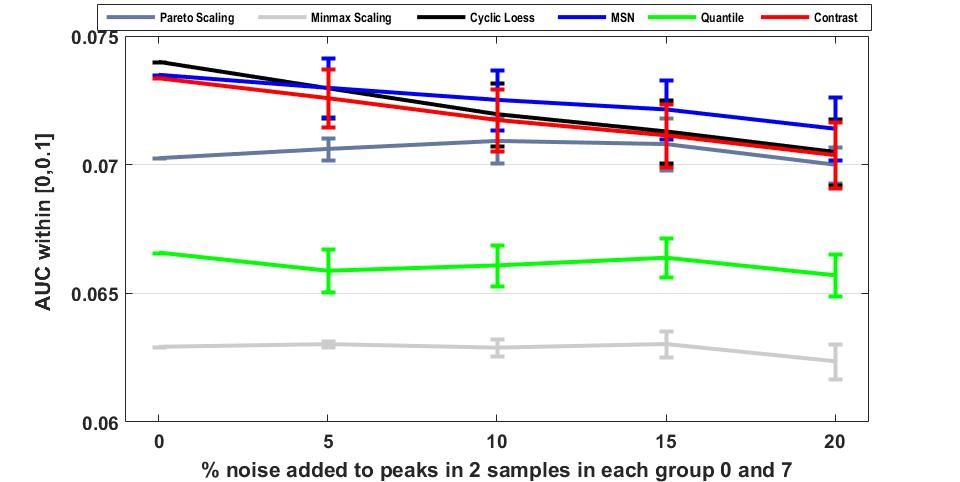
\includegraphics[width=1\textwidth]{g0-7_errorbar}
	\caption{Comparison of the performance of the proposed MSN methods to 5 normalization methods as we vary the noise level and the samples affected by noise in G0 and G7 in the Human Urine Data.}
	\label{g07errorbar}
\end{figure}
\begin{figure}
	
	\centering
	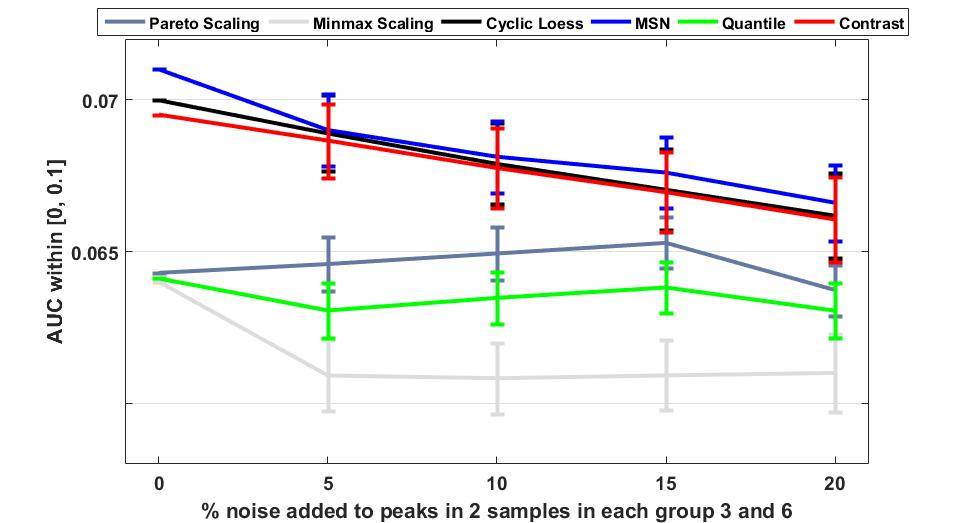
\includegraphics[width=1\textwidth]{g3-6_errobar}
	\caption{Comparison of the performance of the proposed MSN methods to 5 normalization methods as we vary the noise level and the samples affected by noise in G3 and G6 in the Human Urine Data.}
	\label{g36errobar}
\end{figure}
For the second data set, we performed similar experiments as with the metabolomics data set. First, we considered groups $G0$ and $G7$, normalized the data, and used the PLS-DA  to assign a confidence value indicating the likelihood of each feature to be a biomarker. Then, using these confidence values and the ground truth, we computed the area under the curve (AUC) within $[0 \ldots 0.1]$. For this experiment, we corrupted two samples from $G0$ and two samples from $G7$ with multiplicative noise. The corrupted samples were chosen randomly. As with the metabolomics data, we repeated each normalization 10 times and reported the mean and standard deviations of the AUC. The results are shown in Figure ~\ref{g07errorbar}.


As it can be seen, the proposed MSN normalization outperforms other methods as it has the largest AUC values at all noise levels.
In another validation test, we added noise to two samples from group $G0$ and two samples from group $G3$ and repeated the same experiment. The results are shown in Figure ~\ref{g36errobar}, where the same conclusion can be observed.

\section{Evaluation of the proposed Outlier Detection Algorithm}

We used LC-MS metabolomics data to validate the proposed outlier detection method. First, we considered groups $G0$ and $G5$ as it is the easiest case and applied our outlier detection algorithm based on Fisher Criterion. Second, we applied feature selection algorithms to assign a confidence value showing the likelihood of each metabolite to be a biomarker. Using these confidence values and the ground truth, we generated an ROC curve and computed the area under the curve (AUC). Next, we corrupted one or more of the samples from $G0$ and $G5$ by adding outliers to those samples. For a selected samples we added or subtracted a multiple number of sigmas $ k \times \sigma$ with sigmas the standard deviations of each molecule in that group. We will try different values of $k$ and different number of corrupted samples. \\
\indent In TABLE \ref{fld} we report the Area Under the Curve of the classification using the Ensemble Feature Selection method \cite{ali} of $G0$ and $G5$ before and after applying our proposed outlier detection method. 

\begin{table}[h!]
	\centering
	\caption{AUC of Classification Results of $G0$ and $G5$ of Noisy Data after applying our proposed method}
	\begin{tabular}{|c|c|c|c|} 
		\hline
		\textbf{Applied Noise} & \textbf{AUC After ODFC} & \textbf{AUC After OD using Boxplot} &	\textbf{AUC Before OD} \\ [0.5ex] 
		\hline\hline
		\textbf{2 outliers, N= 3$\sigma$
		} & 0.0909 & 0.0840 & 0.0800 \\
		\hline
		\textbf{3 outliers, N= 3$\sigma$
		} & 0.0815 & 0.0775 & 0.0773 \\
		\hline
		\textbf{4 outliers, N= 3$\sigma$} & 0.0741 & 0.0647 & 0.0647\ \\
		
		\hline
		\textbf{3 outliers, N= 4$\sigma$} & 0.0814 & 0.0677 & 0.0681\\
		\hline
		\textbf{4 outliers, N= 4$\sigma$} & 0.0563 & 0.0360 & 0.0353 \\ 
		\hline
	\end{tabular}
	\label{fld}
\end{table}


\begin{table}[h!]
	\centering
	\caption{AUC of Classification Results of $G0$ and $G3$ of Noisy Data after applying our proposed method}
	\begin{tabular}{|c|c|c|c|} 
		\hline
		\textbf{Applied Noise} & \textbf{AUC After ODFC} & \textbf{AUC After OD using Boxplot} &	\textbf{AUC Before OD} \\ [0.5ex] 
		\hline\hline
		\textbf{2 outliers, N= 3$\sigma$
		} & 0.0708  & 0.0674 & 0.0662\\
		\hline
		\textbf{3 outliers, N= 3$\sigma$
		} & 0.0545 & 0.0518 & 0.0491 \\
		\hline
		\textbf{4 outliers, N= 3$\sigma$} & 0.0411  & 0.0392 & 0.0378 \\
		
		\hline
		\textbf{3 outliers, N= 4$\sigma$} & 0.0545  & 0.0518 & 0.0491\\
		\hline
		\textbf{4 outliers, N= 4$\sigma$} & 0.0547 & 0.0368 & 0.0366	 \\ 
		\hline
	\end{tabular}
	\label{fld2}
\end{table}


As it can be seen, after applying the proposed outlier detection method, the AUC has increased in all the experiments. Since the classification accuracy is very high (perfect classification will result in AUC=0.1), the improvement is not very significant. Thus, we can conclude that, the removal of the outliers using the proposed method has improved the performance of the classification.\\
\indent We performed a second experiment, similar to the first one, except that we used groups $G0$ and $G3$ and we measure the AUC of the classification using the Ensembe Feature Selection algortihm \cite{ali}.The results are reported in TABLE \ref{fld2} where a similar conclusion can be observed. In fact, for this harder case, there is more room for improvements and our outlier detection algorithm improved the classification more than the previous experiment.

